% \newpage
\section{Experiments}\label{Sec:experiments}
%%%%%%%%%%%%%%%%%%%%%%%%%%%%%%%%%%%%%%%%%%%%%%%%%%%%%%%%%%%%%%%%%%%%%%%%
A simulation environment was created in RViz in order to test the aforementioned methodologies.
\subsection*{Visual}
The goal of question 1 is to improve upon the existing segmentation algorithm and to make it execute faster. As mentioned in section \ref{Sec:methvis}, three types of filters are tested and analysed against their effects on execution time and segmentation accuracy are also compared with the case where no filter is applied (NON). For question 1.1, VoxelGrid (VG) and StatisticalOutlierRemoval (SOR) are used. For question 1.2, a PassThrough filter (PT) is used based on the question description. The resulting point cloud can be found in fig. \ref{fig:t1}. 

\begin{figure}[h!]
    \centering
    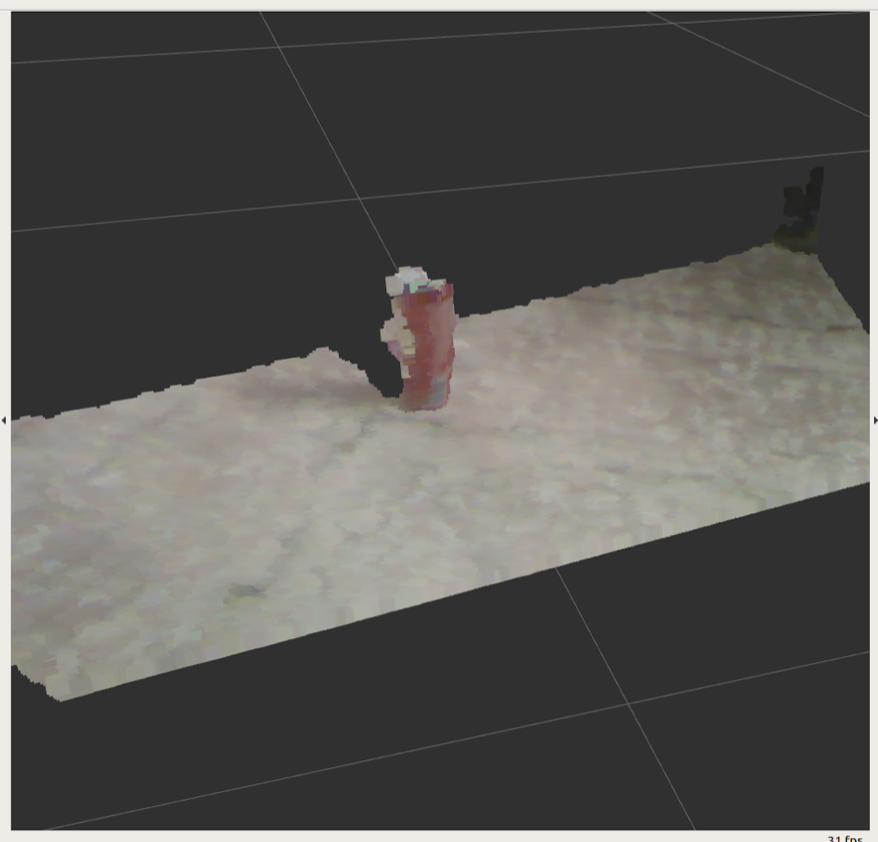
\includegraphics[width=.2\textwidth]{Images/non.png}
    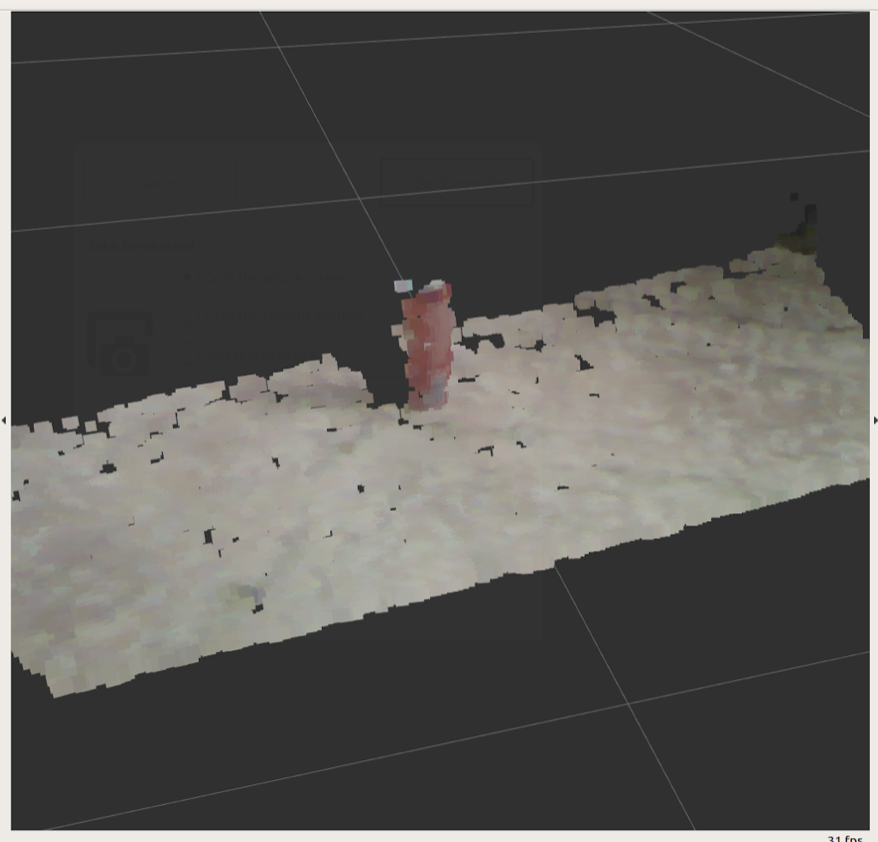
\includegraphics[width=.2\textwidth]{Images/1.1.png}
    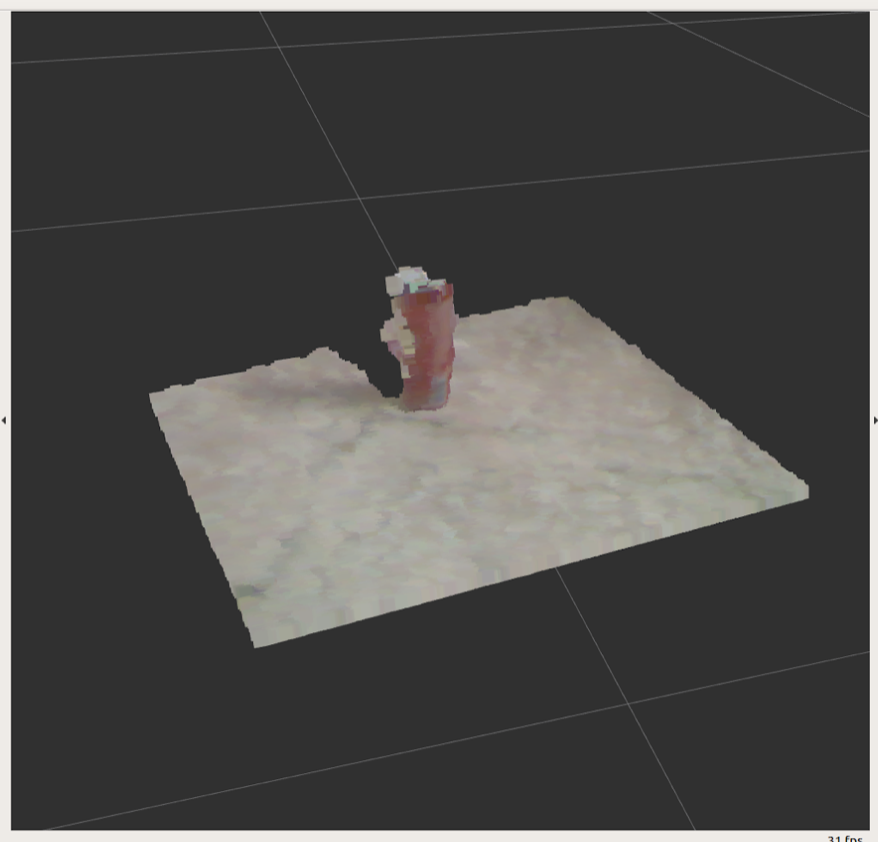
\includegraphics[width=.2\textwidth]{Images/1.2.png}
    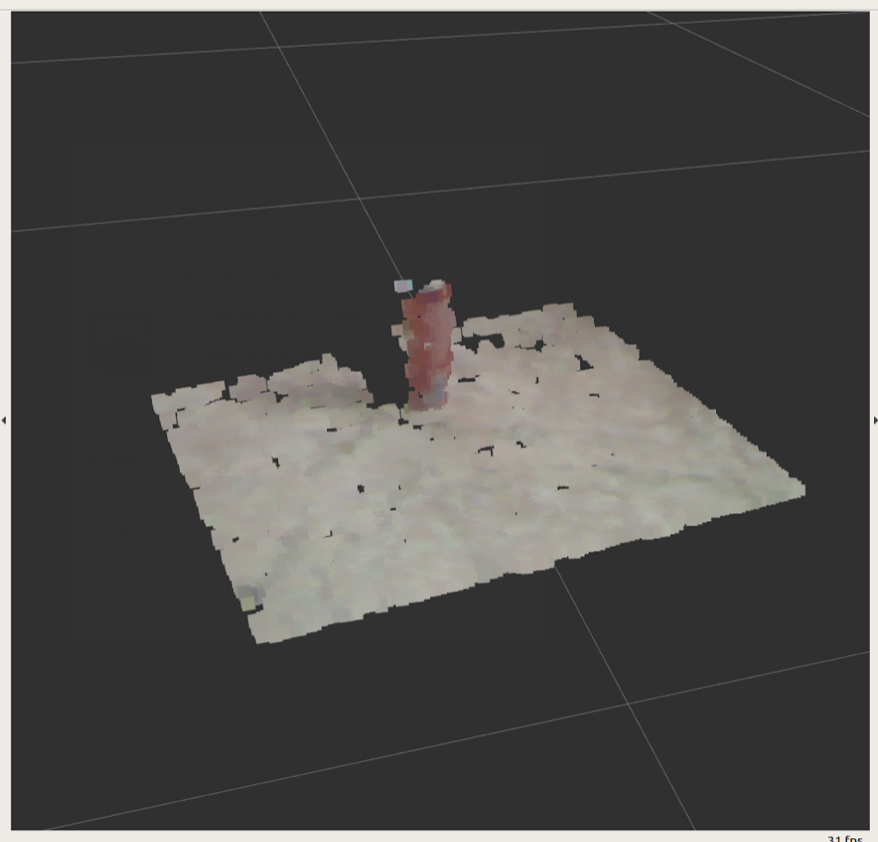
\includegraphics[width=.2\textwidth]{Images/both.png}
    \caption{Filtered PointCloud; top left: no filter; top right: with filters in q1.1; bottom left: with filters in q1.2; bottom right: with filters in both q1.1 and q1.2}
    \label{fig:t1}
\end{figure}

\subsubsection*{Time}
The time consumption of applying filter, segmentation and the total of the two are recorded for different combinations of filters. The following table shows the average time for each filtering function over a randomly-chosen 10 consecutive seconds.
\begin{table}[h!]
\begin{center}
 \begin{tabular}{|c c c c|}
 \hline 
 time(ms) & filtering &  segmentation & total \\
 \hline 
 NON &  24.9 &  634.3 &  659.2\\
 \hline 
 VG &  43.4 &  174.8 &  218.2\\
 \hline 
 SOR &  411.6&  459.1 &  870.7\\
 \hline 
 VG+SOR &  146.2 &  138.7 &  284.9 \\
 \hline 
 PT &  43.1 &  361.2&  404.3 \\
 \hline 
 VG+SOR+PT &  146.1 &  64.4 &   210.5\\
  \hline 
 VG+PT &  48.6 &  92.9 &  141.5 \\
 \hline
\end{tabular}
\end{center}
\caption{time performance of different filtering algorithms}
\label{table:1}
\end{table}

From here we can conclude the following:
\begin{itemize}
    \item in terms of improvement of segmentation performance, the combination of all three filter works the best with the result being 10.15\% of the original time.
    \item in terms of improvement of total performance, counting filtering and segmentation, the combination of VG and PT works the best, with the result being 21.47\% of the original time.
    \item there's a trade-off between the improvement of segmentation performance and using filtering algorithms. More complicated filtering could results in better segmentation performance but meanwhile longer filtering time. 
    \item because the goal of the coursework is to improve the segmentation performance, both SOR and VG are included in question 1.1. 
\end{itemize}

\subsubsection*{Accuracy}
To assess the accuracy of the segmentation. The resulting cylinder pose and size after applying each filter combination are compared against the pose and size when no filter is applied. The following table shows the average results for each filtering function over a randomly-chosen 10 consecutive seconds.

\begin{table}[h!]
\begin{center}
 \begin{tabular}{|c c c c c c|}
 \hline 
 meters & radius &  height & centre x & centre y & centre z \\
 \hline 
 NON &  0.030 &  0.120 & -0.052 & 0.157 &  0.934 \\
 \hline 
 VG &  0.029 &  0.119 &  -0.050 & 0.156 & 0.933\\
 \hline 
 SOR &   0.028 & 0.121 & -0.053 & 0.157 & 0.934 \\
 \hline 
 VG+SOR & 0.025  & 0.121 & -0.055 &0.154 & 0.935\\
 \hline 
 PT &  0.028 & 0.121 & -0.049 & 0.158 &  0.933\\
 \hline 
 VG+SOR+PT &  0.024  &  0.119 & -0.058 & 0.155 & 0.935 \\
  \hline 
 VG+PT &   0.032 & 0.119 & -0.050 & 0.156 & 0.933 \\
 \hline
\end{tabular}
\end{center}
\caption{resulting cylinder position and size of different filtering algorithms}
\label{table:1}
\end{table}

Although we do not have a strict metric for comparing accuracy in terms of the size and position of the resulting cylinder, by roughly looking at the numbers we can see that VG works best when estimating the size of the cylinder and SOR works best when estimating the position of the cylinder. The more complex the filtering algorithms are, the more inaccurate the estimation of cylinder is. Two of the best performing filter combination in terms of time complexity performs relatively poorly here. 

\subsubsection{Conclusion}

From the comparison between different filtering algorithms on their time and accuracy performance, we can see a clear trade-off between the two. More complex combination of filters could result in faster segmentation but less accuracy result and vice versa. 

%%%%%%%%%%%%%%%%%%%%%%%%%%%%%%%%%%%%%%%%%%%%%%%%%%%%%%%%%%%%%%%%%%%%%%%%
\subsection*{Motion}
After the cylindrical object is grasped, only information is coming from the bumper sensors, no further motion capture system is used. In order test the performance of the bumper sensors and the pick and place process several experiments were made where the motion was controlled by the '1', '2' and '3' keys. The experiments of the bumpers can be said successful if they change accordingly and immediately when an object is put or lifted up from the table, which was examined by checking the published Boolean values on the appropriate topics. The performance of the grasp and transportation of the objects is evaluated by executing several different combinations of pick and place tasks and the number of successful attempts are counted. The Franka Emika Panda robotic arm can be seen during a pick and place task on Figure \ref{fig:cylindrical grasp}.


First, the pick and place process of the cylindrical object was tested. By pressing one, the cylindrical object was grasped by a top grasped and placed on the first table.    

\begin{figure}[h]
    \centering
    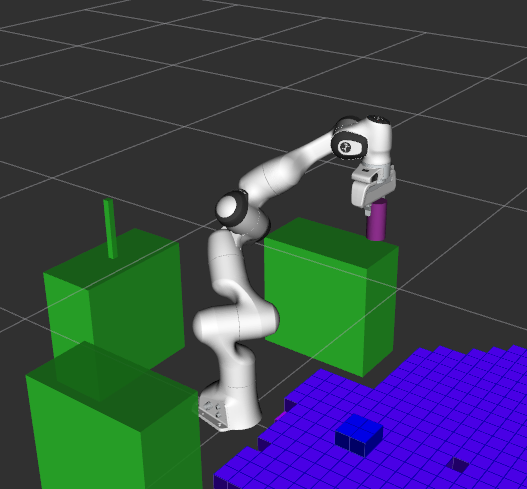
\includegraphics[width=8cm]{Images/cylindrical_grasp.png}
    \caption{A successful top grasp of the cylindrical object, purple highlights that the object is being grasped}
    \label{fig:cylindrical grasp}
\end{figure}

Then, a more complex process was tested. By pressing '2', the robot had to identify from the bumper sensors that table two is occupied; therefore, the robotic arm first needed to place the cubic object to a free table and then, the cylindrical object was moved. Figure \ref{fig:task 2} shows the scene after the aforementioned task was finished.

\begin{figure}[h]
    \centering
    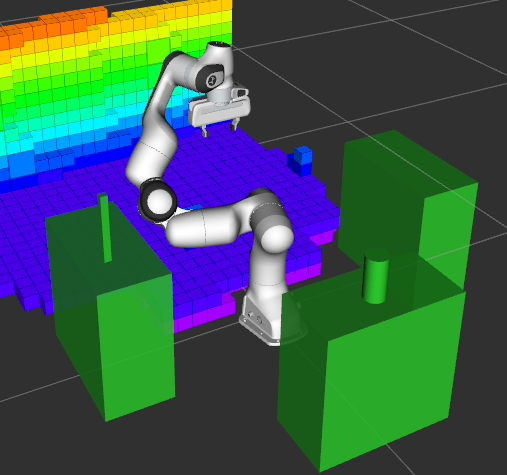
\includegraphics[width=8cm]{Images/task2.png}
    \caption{A Finished, successful task 2}
    \label{fig:task 2}
\end{figure}

Next, further experiments were made; for instance, the transportation of the cylindrical object to the third table and the placement of the cylindrical object to different tables when it is off the ground were executed. During all the attempts, the relevant bumper topics were examined. It can be said that the sensors work properly and detect the changes immediately. 

Overall, the experiments were , and it can be said that the implemented method fulfils the requirements. 